\documentclass{article}
\usepackage{fullpage,color,pgf,tikz}
\usepackage{authblk}
\title{Logic behind the bitsets used for updating diploids in multilocus simulations.  This document is \texbf{not} library documentation and is not intended to make sense to library users.  It is here to remind me what a particularly terse block of code does.}
\author[1]{Kevin R. Thornton}
\affil[1]{Department of Ecology and Evolutionary Biology, UC Irvine}
\date{}
\begin{document}
\maketitle
\section*{Intro}
This document is my reminder of the setup and logic behind the code to generate the next generation's diploids in multilocus simulations.
\section*{The setup}

Simulations of multiple partially-linked loci require that we take two parents, recombine their genomes, and then create a new diploid.  In these simulations, parents are represented as vectors of pairs of iterators to gametes.  Each pair is the parent's genotype at a particular locus, and we allow for partial linkage between each locus.  This scheme is cartooned in Figure \ref{concept}.

\begin{figure}[!h]
  \centering
  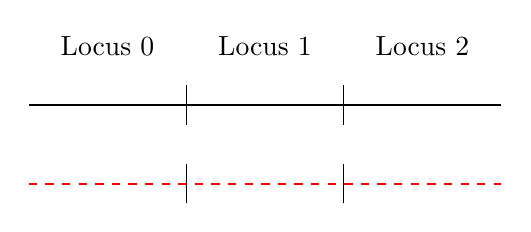
\begin{tikzpicture}
    %locus labels
    \draw (1,2) node[above]{Locus $0$}; 
     \draw (3,2) node[above]{Locus $1$};
    \draw (5,2) node[above]{Locus $2$};
    % p1g1
    \path[draw,thick](0,1.5) -- (6,1.5);
    \path[draw](2,1.25)--(2,1.75); 
    \path[draw](4,1.25)--(4,1.75);
    
    % p1g2
    \path[draw,color=red,dashed,thick](0,0.5) -- (6,0.5);
    \path[draw](2,0.25)--(2,0.75);  
    \path[draw](4,0.25)--(4,0.75);
  \end{tikzpicture} 
  \caption{\label{concept}Conceptual representation of multiple loci.  Shown is a diploid genotype for 3 loci labeled 0 through 2.  Black and red dashed lines represent alleles for each locus (paternal and maternal, for example).  Vertical lines separate the three loci and we imagine that recombination may happen at these vertical lines at some rate.}
\end{figure}

It is a trivial matter to generate the recombinant gametes using existing \texttt{fwdpp} routines.  For example, if there is no crossover between the three loci (\textit{e.g.}, the rates at the two vertical bars in Figure \ref{concept} are all zero), then recombination in on parent may lead to a situation like that shown in Figure \ref{simple}.  After the recombination event, we can simply pick either the top or botom ``row'' of scrambled gametes in Figure \ref{simple} with probability $1/2$ each and choose that row to be passed on to the next generation.
  

\begin{figure}[!h]
  \centering
  \begin{tikzpicture}
    % p1g1
    \path[draw,thick](0,1.5) -- (1,1.5);
    \path[draw,color=red,dashed,thick](1,1.5) -- (3,1.5);
    \path[draw,thick](3,1.5) -- (5,1.5);
    \path[draw,color=red,dashed,thick](5,1.5) -- (6,1.5);
    \path[draw](2,1.25)--(2,1.75); 
    \path[draw](4,1.25)--(4,1.75);
    
    % p1g2
    \path[draw,color=red,dashed,thick](0,0.5) -- (1,0.5);
    \path[draw,thick](1,0.5) -- (3,0.5);
    \path[draw,color=red,dashed,thick](3,0.5) -- (5,0.5);
    \path[draw,thick](5,0.5) -- (6,0.5);
    \path[draw](2,0.25)--(2,0.75);  
     \path[draw](4,0.25)--(4,0.75);
  \end{tikzpicture} 
  \caption{\label{simple}Odd number of crossovers within loci 0 and 1.  No crossover between the loci.}
\end{figure}

Things get a little more complex when crossovers within \textit{and} between loci are occurring.  Figure \ref{xo} shows what we want parental gametes to look like after recombination in a more complex case.

\begin{figure}[!h]
  \centering
  \begin{tikzpicture}
    % p1g1
    \path[draw,thick](0,1.5) -- (1,1.5);
    \path[draw,color=red,dashed,thick](1,1.5) -- (2,1.5);
    \path[draw,thick](2,1.5) -- (3,1.5);  
     \path[draw,color=red,dashed,thick](3,1.5) -- (5,1.5);  
     \path[draw,thick](5,1.5) -- (6,1.5); 
     \path[draw](2,1.25)--(2,1.75);  
     \path[draw](4,1.25)--(4,1.75);
    
    % p1g2
    \path[draw,color=red,dashed,thick](0,0.5) -- (1,0.5);
    \path[draw,thick](1,0.5) -- (2,0.5); 
    \path[draw,thick,color=red,dashed](2,0.5) -- (3,0.5);  
    \path[draw,thick](3,0.5) -- (5,0.5);  
    \path[draw,color=red,dashed,thick](5,0.5) -- (6,0.5); 
    \path[draw](2,0.25)--(2,0.75);  
    \path[draw](4,0.25)--(4,0.75);
  \end{tikzpicture} 
  \caption{\label{xo}Odd number of crossovers within loci 0 and 1.  Crossover between 0 and 1.}
\end{figure}

The question is how to generate outcomes like Figure \ref{xo} efficiently.
\section*{The solution}
We will consider adjacent loci $i$ and $j$, which are two loci out of the $k$ being simulated.  $0 \leq i < k$ and $j = i+1$.  Conceptually, we need to march through the loci and convert something looking like Figure \ref{simple}, which is the output of applying standard per-locus policies already existing in \texttt{fwdpp} to something looking like Figure \ref{xo}, which accounts for the partial linkage between at $k-1$ positions.

We need the following to accomplish this:
\begin{enumerate}
\item If the output of our algorithm (using  Figure \ref{xo} as a concrete example) comes from parent 1, we need to know if we are going to pick ``parent 1, gamete 1'' (p1g1):
  \begin{tikzpicture}
    % p1g1
    \path[draw,thick](0,0.25) -- (1,0.25);
    \path[draw,color=red,dashed,thick](1,0.25) -- (2,0.25);
    \path[draw,thick](2,0.25) -- (3,0.25);  
     \path[draw,color=red,dashed,thick](3,0.25) -- (5,0.25);  
     \path[draw,thick](5,0.25) -- (6,0.25); 
     \path[draw](2,0.)--(2,0.5);  
     \path[draw](4,0.)--(4,0.5);
   \end{tikzpicture}
or ``parent 1, gamete 2'' (p1g2):
  \begin{tikzpicture}
    % p1g2
    \path[draw,color=red,dashed,thick](0,0.25) -- (1,0.25);
    \path[draw,thick](1,0.25) -- (2,0.25); 
    \path[draw,thick,color=red,dashed](2,0.25) -- (3,0.25);  
    \path[draw,thick](3,0.25) -- (5,0.25);  
    \path[draw,color=red,dashed,thick](5,0.25) -- (6,0.25); 
    \path[draw](2,0.)--(2,0.5);  
    \path[draw](4,0.)--(4,0.5);
  \end{tikzpicture} 
as the object that will be inherited.  Conceptually this is trivial, as we are just modeling recombination on a larger scale, then picking one of the gametes at random to pass on.  This choice is represented as a boolean \texttt{p1g1} which is true or false with probability 0.5.
\item At locus $j$, we need to know
  \begin{enumerate}
  \item If the gamete taken from locus $i$ corresponded to parental gamete 1 or 2.  We store this information in a variable called \texttt{LW} (``last was'').  This is an integer taking on values 0 or 1 (for parental gamete 1 and 2, respectively).
  \item If the number of crossover events at locus $i$ was odd or even.  We store this in an integer called \texttt{NR}, which taken on values 0 (odd) or 2 (even).  If \texttt{LW} equals 0, and \texttt{NR} is odd, then the multilocus genotype should be updated with gamete 2 unless there is a crossover between loci (Figure \ref{logic}).
  \item If there is a crossover between $i$ and $j$.  The information is stored in an integer that we will call \texttt{XO}.  \texttt{XO} takes on values 0 (false) or 4 (true).
  \end{enumerate}
\end{enumerate}
The above three variables define a bit set which can take on values 0 through 7.

\begin{figure}[!h]
  \centering
  \begin{tikzpicture}
    % p1g1
    \draw (2,3) node[above]{$i$}; 
    \draw (4,3) node[above]{$j$};
    \draw(0.5,3) node[left]{\texttt{LW}=0,\texttt{NR}=0};
    \path[draw,thick](1,3) -- (3,3); 
    \path[draw,dashed,thick](3,3) -- (5,3);
    \path[draw,thick,color=red](1,2) -- (3,2); 
    \path[draw,dashed,thick,color=red](3,2) -- (5,2);
    
    \draw (6,2.75) node[above]{\texttt{XO}=0};
    \draw[->]  (5.5,2.5) -- (6.5,2.5);
    \path[draw,thick](7,3) -- (9,3); 
    \path[draw,dashed,thick,color=red](9,3) -- (11,3);
    \path[draw,thick,color=red](7,2) -- (9,2); 
    \path[draw,dashed,thick](9,2) -- (11,2);

    \draw (6,1.25) node[left]{\texttt{XO}=1};
    \draw[->]  (5.5,2) -- (6.5,1);
    \path[draw,thick](7,1.5) -- (9,1.5); 
    \path[draw,dashed,thick](9,1.5) -- (11,1.5);
    \path[draw,thick,color=red](7,0.5) -- (9,0.5); 
    \path[draw,dashed,thick,color=red](9,0.5) -- (11,0.5);
  \end{tikzpicture} 
  \caption{\label{logic}The logic for updating}
\end{figure}
\end{document}
